\documentclass[11pt]{beamer}
\usepackage[utf8]{inputenc}
\usepackage[T1]{fontenc}
\usepackage{lmodern}
\usepackage{amsfonts}
\usepackage{amsmath}
\usepackage{amssymb}
\usepackage{ragged2e}
\usepackage{graphicx}
\usepackage{natbib}
\usetheme{Madrid}
	\author{Ruben ESPELETA BOLIVAR}
\title[Numerical experiments]{Numerical experiments in idealized glacier topographies}
\date{May 24th, 2023}

\subtitle{Case study of the impact of the mesh resolution on the prediction of the grounding line position}
\logo{
\includegraphics[scale=0.15]{../fig/logo_IGE.png}}
\institute[IGE]{
	\inst{1}
	Institut des geosciences de l'environnement
}
%\subject{}
%\setbeamercovered{transparent}
%\setbeamertemplate{navigation symbols}{}
\AtBeginSection[]{
	\begin{frame}<beamer>{Contenido}
		\tableofcontents[currentsection]
	\end{frame}
}
\begin{document}

	\begin{frame}
		\maketitle
	\end{frame}
	
	\begin{frame}{Content}
		\tableofcontents
	\end{frame}
	
	\section{Introduction}
	\subsection{Definition}
		\begin{frame}{Definition}
		\justifying
		Glaciers can be defined as a mass of ice that accumulates from snow and flows slowly downwards
		\begin{figure}
		\centering
		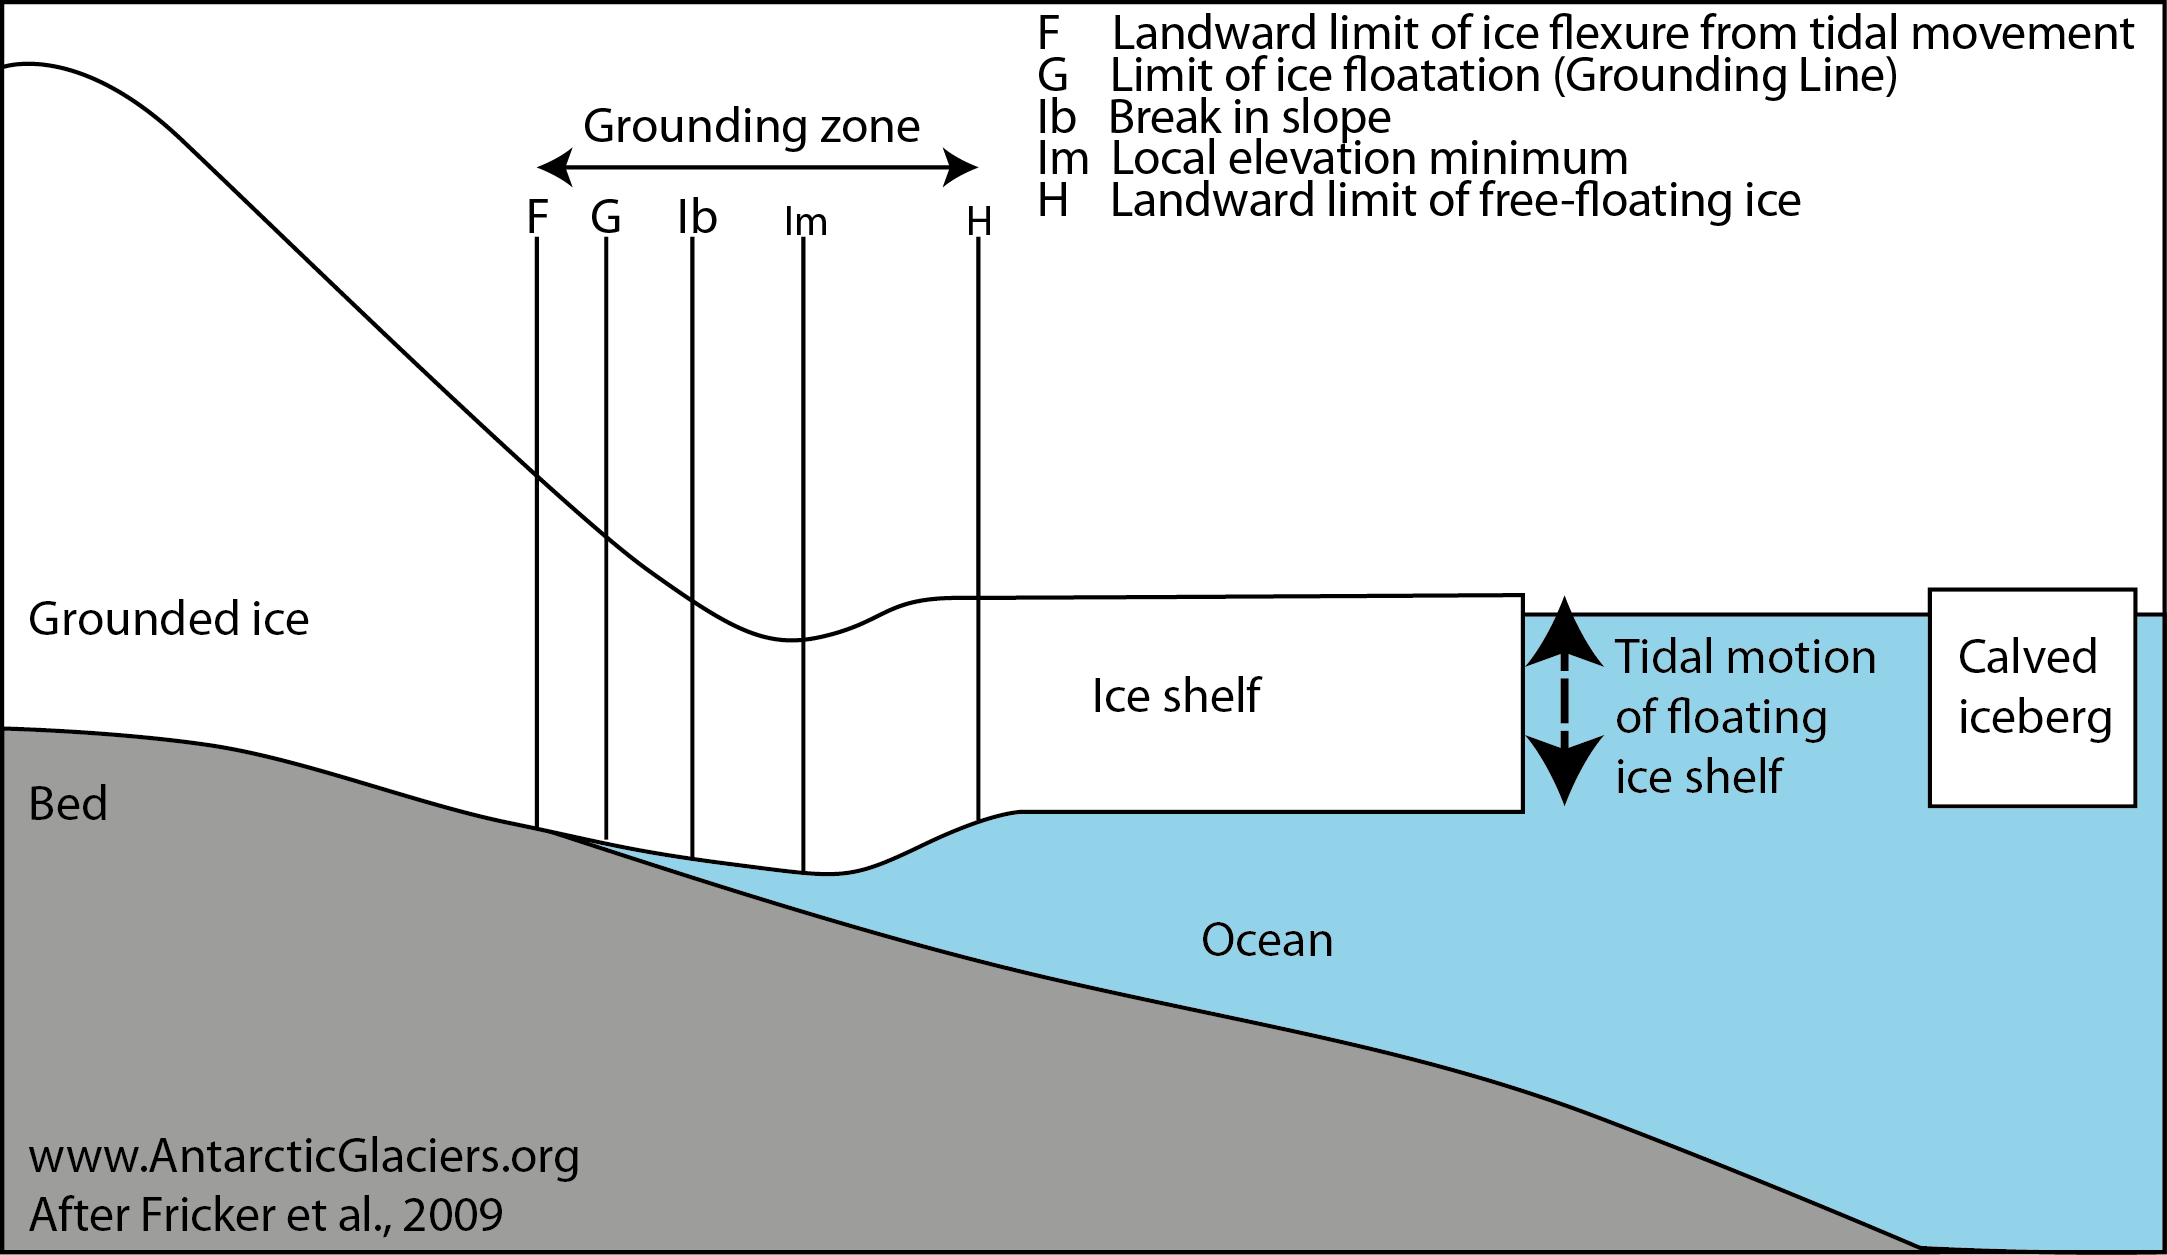
\includegraphics[scale=0.4]{../fig/groundingzone.png}
		\caption{Schema of a tributary glacier where we can observe the different parts denoting the grounding zone \cite[]{fricker2009mapping}. Adapted from AntarticGlaciers.org}
		\label{Glacier}
		\end{figure}
		\end{frame}

	\subsection{Importance of understanding the dynamics of glaciers}
		\begin{frame}{Importance of understanding the dynamics of glaciers}
		\justifying
		\begin{itemize}
			\item The rate of present-day sea-level rise has increased in recent decades and it is expected to continue increasing in coming decades and centuries \cite[]{clark2015recent}.
			\item \cite{morlighem2017bedmachine} and \cite{haywood2011pliocene} mentioned that if all the ice were to melt completely, the sea level would rise by an estimated of 65m.
			\item The Unites Nations states that around 40\% of the world's population lives in coastal regions, within 100km of the coastline \cite[]{barbier2015climate, montgomery2007united}.
			\item The land area that is less than 10m above sea level is just 2\% of the world's total land area, yet it is home to 10\% of the world's population and 13\% of the world's urban population \cite[]{nevermann2023land}.
		\end{itemize}
		\end{frame}
	\section{Glacier dynamics}
	\subsection{Mass flux}
		\begin{frame}{Mass flux}
		\justifying
		The velocity out in the x-direction is:
		\begin{equation}
			U = u+\frac{\delta u}{\delta x}dx;
		\end{equation}
		\begin{figure}
			\centering
			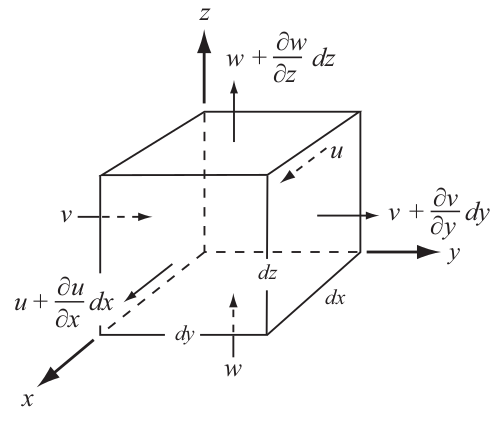
\includegraphics[scale=0.2]{../fig/Control_volume.png}
			\caption{Derivation of the condition of incompressibility. Adapted from \cite{hooke2019principles}.}
			\label{control_volume}
		\end{figure}
		\end{frame}
	\subsection{Incompessibility condition}
		\begin{frame}{Incompressibility condition}
		\justifying
		Mass fluxes into and out of a elementary control volume of ice in a glacier in the x-direction are:
		\begin{equation}
			({\rho u + \frac{\delta \rho u}{\delta x}dx})dy dz;
		\end{equation}
		Here, $\rho$ is the density of the ice. Similar relations may be written for the mass fluxes into and out of the volume control in the $y$ and $z$-directions. Summing these fluxes we find that the change in mass with time, $\frac{\delta m}{\delta t}$ in the control volume is:
		\begin{equation}
			-\frac{1}{dxdydz}\frac{\delta m}{\delta t}=\frac{\delta \rho u}{\delta x}+\frac{\delta \rho v}{\delta y}+\frac{\delta \rho w}{\delta z};
		\end{equation}
		The mass of ice in the control volume can change if the control volume is not full initially. When it is full of incompressible ice, however, $\frac{\delta m}{\delta t}=0$, and the equation becomes:
		\begin{equation}
			\frac{\delta u}{\delta x}+\frac{\delta v}{\delta y}+\frac{\delta w}{\delta z}=0;
		\end{equation}
		\end{frame}
	\subsection{Deviatoric stress}
		\begin{frame}{Deviatoric stress}
		\justifying
		The deviatoric normal stress in the x-direction is:
		\begin{equation}
			\sigma_{XX}'= \sigma_{XX}-P;
		\end{equation}
		Where P is the mean normal stress:
		\begin{equation}
			P=-\frac{1}{3}({\sigma_{XX}+\sigma_{YY}+\sigma_{ZZ}})
		\end{equation}
		\begin{figure}
			\centering
			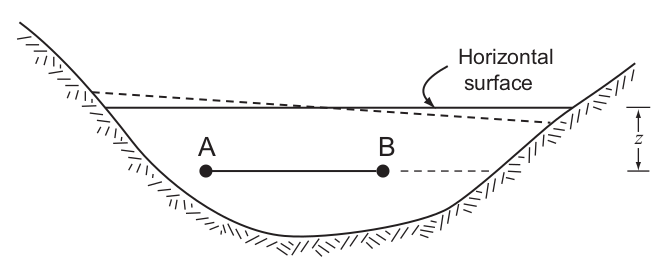
\includegraphics[width=0.4\linewidth]{../fig/Non_hydrostatic_pressure.png}
			\caption{Sketch to illustrate non-hydrostatic pressure. Adapted from \cite{hooke2019principles}.}
			\label{Deviatoric_stress}
		\end{figure}
		\end{frame}
	\subsection{The flow law and governing equations}
		\begin{frame}{The flow law and governing equations}
		\justifying
		The most commonly used flow law for ice is Glen’s flow law, named after John W. Glen upon whose experiments it is based \cite{glen1958flow}. This equation was originally written in the form:
		\begin{equation}
			\dot{\epsilon_{e}}=({\frac{\sigma_{e}}{B}})^n;
		\end{equation}
		where B is a viscosity parameter that increases as the ice becomes stiffer, and n is an empirically determined constant. Most studies have found that n=3¸. An alternative form of the flow law that is commonly used, and that can be used, is:
		\begin{equation}
			\dot{\epsilon_{e}}=A{\sigma_{e}}^n
		\end{equation}
		A is called the rate factor. B is normally given in Mpa yr$^{\frac{1}{n}}$ while A is in MPa$^{-n}$ yr $^{-1}$ or MPa$^{-n}$ s $^{-1}$.
		\end{frame}
	\subsection{Governing equations}
		\begin{frame}[allowframebreaks]{Governing equations}
		\justifying
			\begin{figure}
				\centering
				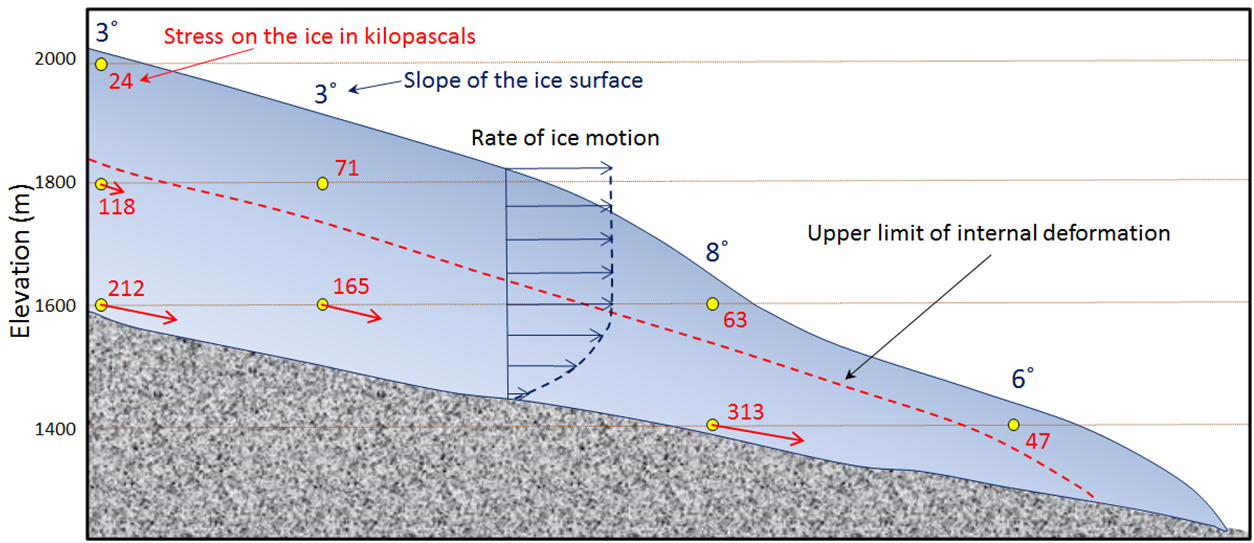
\includegraphics[scale=0.3]{../fig/ice_flow.png}
				\caption{Stress within a valley glacier (red numbers) and the ice velocity (blue arrows). Figure adapted from \cite{earle2015physical}}
				\label{Flow_ice}
			\end{figure}
		The plastic lower ice of the glacier can flow like a very viscous fluid. The incompressibility condition leads to:
		\begin{equation}
			\nabla u=0
		\end{equation}
		For ice flow, the acceleration term can be neglected in the Navier-Stokes equations \cite[]{hutter1982mathematical}. Therefore:
		\begin{equation}
			-\nabla p+\nabla (\eta (\nabla u+(\nabla u)^T))+\rho g = 0;
		\end{equation}
		Where $\eta$ is the viscosity and $g$ is the gravity. Letting $\sigma$ denote the stress tensor and pressure $p$ is the mean normal stress denoted previously, and the strain rate tensor $\epsilon_{e}$, related by:
		\begin{equation}
			\sigma=2\eta \epsilon_{e}-pI = \eta (\nabla u+(\nabla u)^T)-pI; 
		\end{equation}
		Where I is the identity tensor. Together, these two last mathematical equations are called the full-stokes model.
		\end{frame}
		\begin{frame}[allowframebreaks]{Boundary conditions and time evolution}
		\justifying
			\begin{itemize}
				\item Ice in contact with the bedrock: Weertman sliding law \cite[]{weertman1974stability}:
				\begin{equation}
					u_b=C{\tau_b}^m;
				\end{equation}
				\item The ice surface is assummed stress free $\sigma .n=0$ and ice base at $z_s$ and $z_b$ behave as free surfaces according to:
				\begin{equation}
					\frac{\delta z_{s/b}}{\delta t}+u_{s/b}\frac{\delta z_{s/b}}{\delta x}+v_{s/b}\frac{\delta z_{s/b}}{\delta y}=w_{s/b}+a_{s/b};
				\end{equation}
			where $a_{s/b}$ is the accumulation ($a_{s/b}>0$) or ablation ($a_{s/b}<0$) in meter ice equivalent per year, at the surface or at the base, respectively.
			\item By vertical integration of the incompressibility condition, $w$ can be eliminated:
			\begin{equation}
				\frac{\delta H}{\delta t}+\frac{\delta H\bar{u}}{\delta x}+\frac{\delta H \bar{v}}{\delta y}=a_s-a_b ;
			\end{equation}
			Where $\bar{u}$ and $\bar{v}$ are the vertically integrated horizontal velocities. 
			\item For the ice-ocean interface, as soon as the seawater pressure $p_w$ at the ice base $z_b$ is larger than the normal stress exerted by the ice at the bed, the ice is assumed to float. At the ice-ocean interface, the tangential friction is neglected and:
			\begin{equation}
				\sigma  n=-p_wn ;
			\end{equation}
			where:
			\begin{equation}
				p_w(z)=-\rho_wgz; if z<0;
			\end{equation}
			and $\sigma n=0$ above sea level ($z>0$).
			\end{itemize}
		\end{frame}

	\subsection{Shallow shelf approximation}
		\begin{frame}{Shallow shelf approximation}
			Floating ice does not experience basal drag, hence all resistance comes from longitudinal stresses and lateral drag at the margins (figure \ref{nine_stresses}).
			A dimensional analysis shows that vertical variation of in $u$ and $v$ is negligible, such that $w$ and $p$ can be eliminated by integrating the remaining stresses over the vertical and applying the boundary conditions at the glacier surface and base:
			\begin{equation}
				\nabla_h.(2\bar{\eta}(\dot{\epsilon_h}I))=\rho g H \nabla_h z_s;
			\end{equation}
			
		\end{frame}
	\section{Grounding line dynamics and stability}
		\begin{frame}{Grounding line dynamics and stability}
		contenidos...
		\end{frame}

	\section{Numerical model}
	\subsection{Process of modelling}
	\begin{frame}{Process of modelling}
		\justifying
		The physical phenomena that impacts the dynamics of the glaciers can be represented using mathematical models that implement partial differential equations, which can then be discretized to be solved using numerical methods.
		\begin{figure}
			\centering
			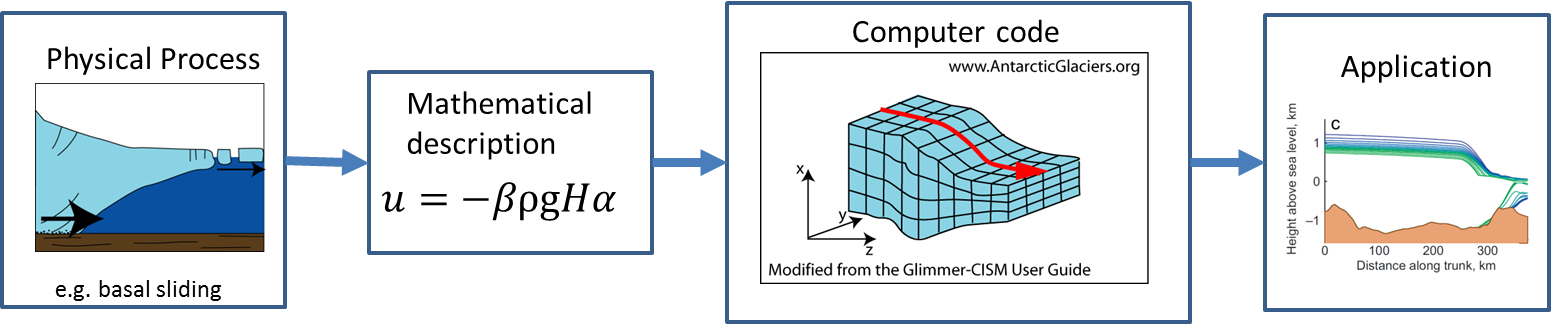
\includegraphics[scale=0.4]{../fig/Numerical_modelling_scheme.png}
			\caption{Process of modelling, starting with a physical phenomena which can be represented mathematically in a physical model than can then be discretized to solve numerically. Adapted from AntarticGlaciers.org}
			\label{Modelling}
		\end{figure}
	\end{frame}
		\begin{frame}{Numerical model}
		contenidos...
		\end{frame}
	\section{Numerical parameters}
		\begin{frame}{Numerical parameters}
		contenidos...
		\end{frame}
	\section{Systems and experiment set-up}
		\begin{frame}{Systems and experiment set-up}
		contenidos...
		\end{frame}
	\section{Results}
		\begin{frame}{Results}
		contenidos...
		\end{frame}
	\section{Conclusions}
		\begin{frame}{Conclusions}
		contenidos...
		\end{frame}
	\section{Bibliography and references}
		\begin{frame}[allowframebreaks]
		\frametitle{Bibliography and references}
			\bibliography{./biblio}
			\bibliographystyle{apalike}
		\end{frame}
\end{document}